\ifx\wholebook\relax \else

\documentclass{article}

\usepackage[nomarginpar
  %, margin=.5in
]{geometry}

\addtolength{\oddsidemargin}{-0.05in}
\addtolength{\evensidemargin}{-0.05in}
\addtolength{\textwidth}{0.1in}

\usepackage[cn]{../prelude}

\setcounter{page}{1}

\begin{document}

\title{悖论}

\author{刘新宇
\thanks{{\bfseries 刘新宇} \newline
  Email: liuxinyu95@gmail.com \newline}
  }

\maketitle
\fi

\markboth{悖论}{编程中的数学}

\ifx\wholebook\relax
\chapter{悖论}
\numberwithin{Exercise}{chapter}
\fi

\epigraph{除了自己的无知,我什么都不懂。}{——苏格拉底}

\begin{wrapfigure}{R}{0.5\textwidth}
 \centering
 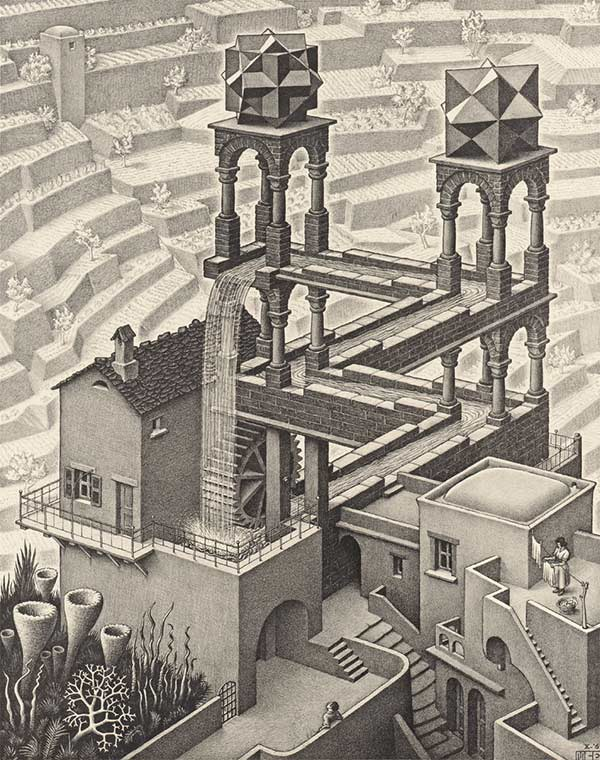
\includegraphics[scale=0.3]{img/Escher-Waterfall-1961.eps}
 \captionsetup{labelformat=empty}
 \caption{埃舍尔《瀑布》1961}
 \label{fig:Escher-Waterfall}
\end{wrapfigure}

\index{深蓝}
1996年,第26界国际奥林匹克运动会正在美国的亚特兰大举行。来自世界各地的选手在速度、力量、技巧上展开竞赛挑战人类的极限。与此同时,还进行着另一场有趣的竞赛。超级计算机“深蓝”与国际象棋世界冠军卡斯帕罗夫展开了对抗赛。比赛结果是深蓝2胜4负输给了人类象棋冠军。翌年,改进的深蓝再次向卡斯帕罗夫发起挑战。5月11日,计算机在正常时限的比赛中首次击败了卡斯帕罗夫。总比分2胜1负3平。深蓝计算机重1270公斤,有32个微处理器,每秒钟可以计算2亿步。为了能让"深蓝”挑战人类冠军,设计小组输入了一百多年来优秀棋手的两百多万个对局。人类用智慧创造的机器,在人类骄傲的智慧领域首次击败了人类自己——这一结局引发了关注、恐惧、和激烈的讨论。

在当时,人们普遍认为,这是人工智能的一大进步。尽管在国际象棋上取得了巨大进步,但是在围棋上,计算机和人类仍存在巨大差距。对于国际象棋来说,棋盘8行8列,32枚棋子。计算机要在$10^{123}$这样巨大的博弈树中进行搜索。即使深蓝美秒能算2亿步,遍历博弈树仍需要近$10^{107}$年。为此深蓝的设计小组通过计算机程序缩小了搜索空间,使得深蓝能够搜索当前棋局后面的12步棋。而一般好的人类棋手,大约只能估计到10步左右。但是围棋的棋盘有19行19列,在一共361个格点上可以放置黑色或者白色的棋子。博弈树的规模为$10^{360}$,远远超越国际象棋。所以在之后的一段时间里,人们仍然不相信计算机可以挑战我们。

%\begin{wrapfigure}{R}{0.5\textwidth}
\begin{figure}[htbp]
 \centering
 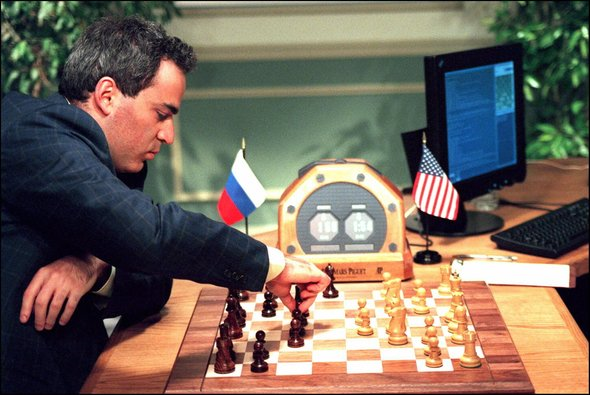
\includegraphics[scale=0.4]{img/Deep-blue-1997.eps}
 \captionsetup{labelformat=empty}
 \caption{卡斯帕罗夫在与深蓝对弈,图片原载《科学美国人杂志》}
 \label{fig:Deep-blue-1997}
\end{figure}
%\end{wrapfigure}

\index{Alpha-Go}
时光匆匆过去了20年,2016年,计算机程序Alpha-Go向人类的围棋大师展开了挑战。韩国的九段棋手李世石以1比4的总比分输掉了比赛。一年后,Alpha-Go再次以3局全胜的成绩战胜了中国棋手柯洁。被人们认为是人工智能游戏“圣杯”的围棋终于被攻破了。面对没有感情的计算机,柯洁心有不甘,潸然落泪。作为人类,我们的心情很复杂。即使是从事智力工作的程序员群体也感到了来自机器的压力——我们是否会被机器取代?

%University of Tubingen, Germany
% Leon A. Gatys, Alexander S. Ecker Matthias Bethge
传统上我们认为,艺术文学等领域,涉及人们的文化背景、内在感情和与生俱来的性格因素,是无法被机器所替代的。2015年,德国斯图加特以南40公里的小镇图宾根大学的盖提斯、埃克、贝特格三位研究人员利用机器学习人类艺术家的风格,把图宾根镇的一张风景照片变换成了不同风格的艺术画作\cite{Gatys-2015}。无论是后印象派大师梵高色彩强烈夸张的画风,还是透纳那浪漫主义水天浑浊的光影效果,都被机器模仿得惟妙惟肖。犹如大师本人所作(图\ref{fig:style-transfer})。

%\begin{wrapfigure}{R}{0.5\textwidth}
\begin{figure}[htbp]
 \centering
 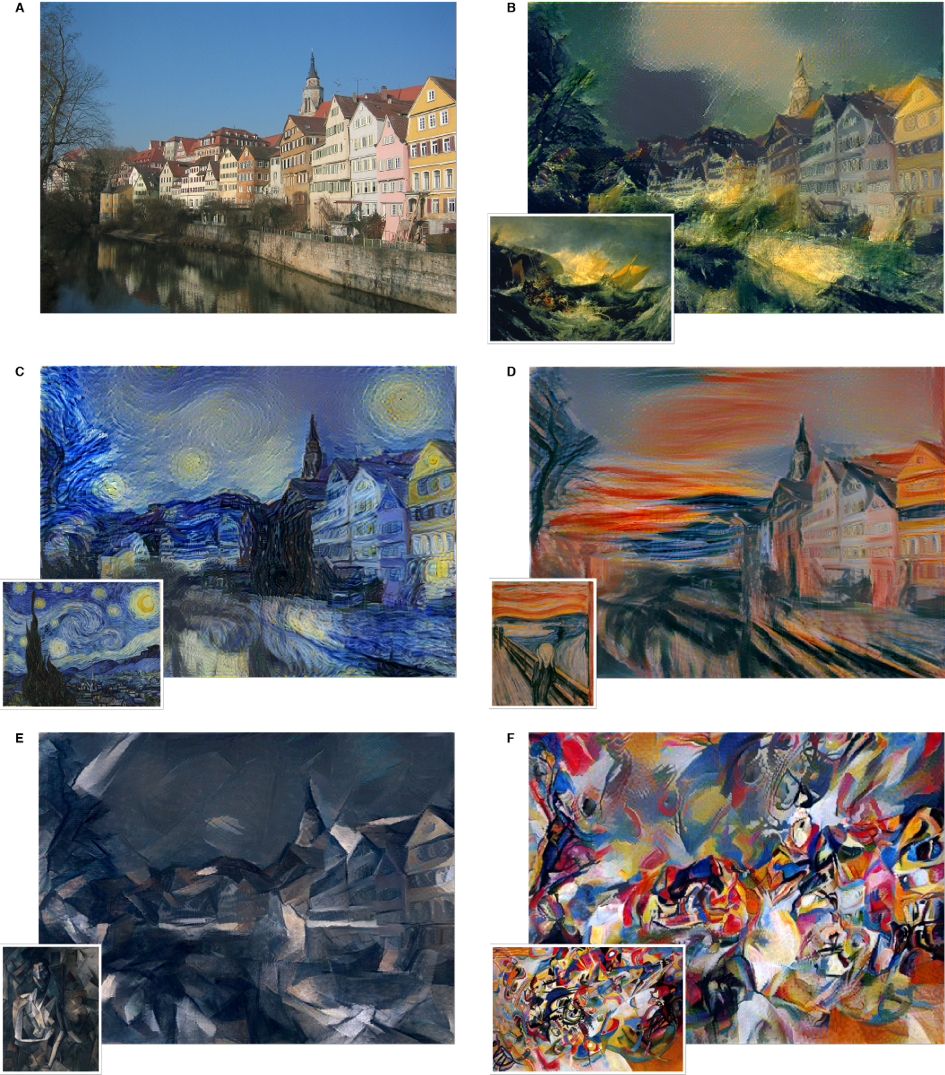
\includegraphics[scale=0.85]{img/style-transfer.eps}
 %\captionsetup{labelformat=empty}
 \caption{机器学习产生的不同艺术风格的画作:A,图宾根镇的风景照片;B,英国画家透纳1805年的原作《运输船遇难》和透纳风格的画作;C,荷兰后印象派画家梵高1889年的原作《星空》和梵高风格的画作;D,挪威表现主义画家爱德华$\cdot$蒙克1893年的原作《呐喊》和蒙克风格的画作;E,西班牙现代艺术家毕加索1910年的原作《坐着的裸女》和毕加索风格的画作;F,俄罗斯抽象艺术先驱画家康定斯基1913年的原作《构成第七号》和康定斯基风格的画作。}
 \label{fig:style-transfer}
\end{figure}
%\end{wrapfigure}

在随后的数年中,人工智能和机器学习突飞猛进地进入了各种领域。机器产生不同音乐家风格的音乐,能够演奏出紧张、舒缓等不同的情绪的旋律和节奏,而不再是呆板单调的电子琴音。机器批量翻译新闻稿和各种学术论文,和专业翻译的文笔不相上下。机器处理X片、CT、核磁共振等医学图像并给出病理诊断,并且结果在准确程度上超越人类医生,人工智能操控的无人车在街道上行驶,成功超过其它车辆并避让行人。无人值守的商店突然出现在街边,人们可以直接从货架上拿走商品,并在走出商店的一刻自动支付……作为人类的我们不禁会问:我们消灭工作岗位的速度是否会超过创造工作机会的速度?人类是否会被机器全面取代?机器是否最终会统治我们?

所有这些在本质上都可以归结到一个问题:计算的能力是否存在边界?如果有的话,计算的边界在哪里?

\section{计算的边界}

顾森在《思考的乐趣》一书中讲到注视着一个运行了很久的程序时的两难心情:这个程序能结束么?是应该继续等下去,还是杀掉进程强行结束?有没有什么编译器能事先告诉你的程序是否会无限运行下去?(\cite{GuSen-2012},第228页)

\begin{quotation}
为什么不可能呢?这个东西看上去比时光旅行机更现实一些。或许我们会在某个科幻电影中看到,一个程序员在漆黑的屏幕上输入几个数,敲了一下回车,然后屏幕上立即用高亮加粗字体显示:“警告:该输入数据会导致程序无限运行下去,确定执行?(Y/N)”如果有一天,这一切真的成为了现实。那么你能利用这个玩意儿来做些什么实用、有价值的事情?如果我说你能靠这玩意儿发大财的话,你相信么?……我上来就先写一个哥德巴赫猜想的验证程序。我写一个程序,让他从小到大枚举所有的偶数,看是不是有两个质数加起来等于它。如果找到了,继续枚举下一个偶数,否则输出反例并结束程序。然后编译该程序。这个编译器不是可以预先判断我这个程序能否终止吗?如果编译器说我这个程序会无限执行下去的话,我岂不是相当于证实了哥德巴赫猜想吗?或者,编译器说程序会最终终止,那哥德巴赫猜想不就直接被推翻了吗?不管怎样,我都将成为解决哥德巴赫猜想的第一人,在数学史上留下自己的名字。接下来呢?把刚才的程序代码改成孪生素数搜索器,在利用编译器检查一下,看看是不是真的有无穷多个孪生素数。梅森素数是否有无穷多个,这个也是数论中长期以来悬而未决的难题。不过现在看来,我也能不费吹灰之力就把它解决了。还记得$3x+1$问题吗?写一个“证明程序”也只是几分钟的事情,而且还能拿走埃尔德什提供的500美元奖金呢。数学上的未解之谜多着呢。我永远不愁没事做。1984年,马丁$\cdot$拉巴尔询问能否用9个不同的平方数构成$3 \times 3$幻方,这个问题的奖金目前已经积累到了100美元加100欧元再加一瓶香槟。网上搜索“数学未解难题”,看看哪些问题是离散的,其中又有哪些问题是有悬赏的,写几个程序就可以把它们统统解决……
\end{quotation}

\index{图灵停机问题}
1936年,计算机科学和人工智能的先驱图灵证明了一个命题:不存在可以判断任何程序是否可以停机的通用算法。证明的核心部分包含了计算机程序的数学定义——图灵机模型。后人称这一问题为图灵停机问题。

为了证明图灵停机问题,我们采用反证法,假设存在一个名叫$halts(p)$的算法,能够判断任意程序$p$是否停机。首先我们定义一个永不停机的程序:

\[
forever() = forever()
\]

这是一个无穷递归的调用。然后我们构造一个名为$G$的特殊程序\footnote{我们用字母$G$是有特殊用意的,$G$是哥德尔的首字母,它恰好和哥德尔不完全定理中不可判定命题的名字相同。},它的定义如下:

\[
G() = \begin{cases}
halts(G) = \text{停机}: & forever() \\
\text{否则}: & \text{停机} \\
\end{cases}
\]

在程序$G$中,我们通过$halts(G)$判断$G$本身是否停机。如果停机,我们就调用$forever()$永远运行下去。但这恰恰说明$G$不会停机,所以$halts(G)$应该为假,但是按照上面定义的第二行,此时我们停机。这恰恰说明$halts(G)$应该为真。所以不论$halts(G)$是真是假,我们都会得到矛盾的结论。因此我们最初的假设不成立,也就是说,不存在一个可以判断任意程序能否停机的通用算法。

也有一种分两步证明图灵停机问题的方法(\cite{SICP},第268页),前面都一样,但在构造$G$时,$G$接受一个参数$p$,它把$p$应用到自身上并传给$halts$:

\lstset{frame=single}
\begin{lstlisting}
G(p) = if halts(p(p)) then forever() else 'Halted'
\end{lstlisting}

接下来的一步中,我们把$G$传给自己$G(G)$看发生了什么?此时如果$halts(G(G))$返回真,则接下来运行$forever()$,所以$G(G)$永远运行不会停机。但这恰恰说明$halts(G(G))$应该返回假,所以接下来程序进入\texttt{else}分支,返回停机。但这又说明$halts(G(G))$应该返回真。所以不管停机与否,都陷入了矛盾之中。

伟大的图灵停机定理清晰地给出了一个不可计算问题。击碎了我们本节中给出的那些奇思妙想。看到这里,你是否想起了上一章附录中康托尔定理的证明?我们用极为类似的方法证明了任何集合,包括无穷集合的势都小于它的幂集的势。实际上,图灵停机问题让我们联想起了一大类有趣的逻辑悖论。

\section{罗素悖论}

% Eubulides of Miletus
悖论从古希腊时期就被人们发现了。上一章我们介绍了关于无穷和连续的芝诺悖论,而逻辑悖论是一类从严密逻辑导出矛盾结果的有趣问题。公元前四世纪,古希腊哲学家米利都的欧歩里德提出这样一个命题:“我现在说的是一句假话”,怎样判断这句话的真伪呢?

如果这句话是假话,那么它陈述的事实(正在说谎)就成了真的,因此矛盾。但如果这句话是真话,那么这句话的原话说正在说谎,因此它是假话,也产生了矛盾。不论欧歩里德说的是真是假,我们都将陷入矛盾中,这一著名的令人困惑的问题被人们称为“说谎者悖论”。

\index{说谎者悖论}
说谎者悖论还有一个两段体的变形,以对话的形式出现。例如:

\textbf{阿基里斯}:乌龟是个狡猾的家伙,总爱说谎,你听,它下面的话就是假的。

\textbf{乌龟}:亲爱的阿基里斯,诚实的你总是说真话。

乌龟的话到底是真是假呢?如果乌龟说了真话,也就是阿基里斯的陈述是真的。但阿基里斯说乌龟在撒谎,这就导致了矛盾。反之如果乌龟说的是假话,那么阿基里斯说的就是假的,于是乌龟说的这就话就应该为真。我们陷入了怪圈,无论乌龟的话是真是假,都会导致矛盾。

这种两段体式的说谎者悖论有时还以恶作剧的形式出现。你收到一张纸条,上面写着“背面是假的”,等你翻到纸条背面,却看到上面赫然写着“背面是真的”。到底哪面是真的呢?仔细分析下来,就会发现陷入了逻辑怪圈。

儿童故事中,也有不少这种悖论。有一则说狮子捉到了兔子,得意地说,如果你能猜中接下来我要干什么,我就放了你,要是猜错了,我就吃掉你。聪明的兔子说:“我猜你要吃掉我。”

如果狮子吃掉兔子,那说明兔子猜中了。这样狮子应该兑现承诺,放掉兔子。可是如果放掉兔子,这说明兔子猜错了。按道理狮子又应该吃掉兔子。狮子陷入了两难处境。既不能吃掉兔子,也不能不吃兔子。估计它只能发疯而让聪明的兔子溜走了。

传说古希腊的军队战胜了波斯,国王决心“优待俘虏”,让他们选择死亡的方式。俘虏可以说一句话,如果是真话,就被砍头,如果是假话,就被绞死。一个聪明的俘虏说:“我猜你要绞死我。”如果国王绞死了俘虏,说明他说了真话,可是这样,按照规则应该被砍头。但如果砍掉他的头,就和这个人讲的内容不符了,所以他说了假话。这样就应该被绞死。结果不论砍头还是绞死,国王的命令都没有被正确的执行。国王万般无奈,不仅释放了这个俘虏,还释放了所有其他人。

\begin{wrapfigure}{L}{0.5\textwidth}
 \centering
 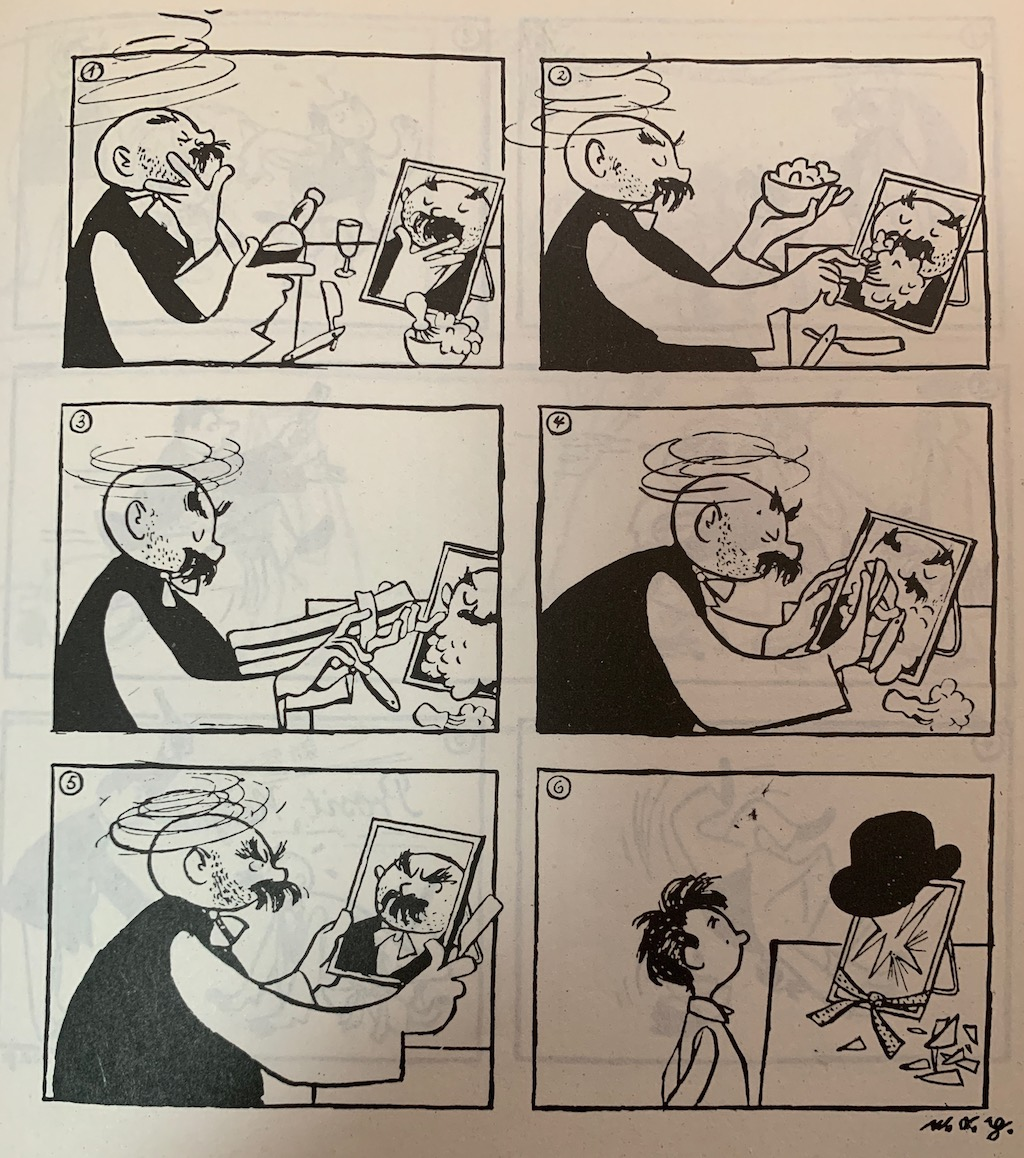
\includegraphics[scale=0.17]{img/father-and-son.eps}
 \captionsetup{labelformat=empty}
 \caption{[德]埃$\cdot$奥$\cdot$卜劳恩《父与子》一则,1930年代}
 \label{fig:father-and-son}
\end{wrapfigure}

塞万提斯在他的伟大作品《堂$\cdot$吉诃德》中,也讲了一个有趣的悖论。有一位贵族的封地被一条大河分成了两半,河上有一座桥,桥的尽头有个绞架。这位贵族制定了一条法令:“过桥的人必须诚实声明他的目的,如果是真话就允许过桥,如果说谎,就判处绞刑,绞死在桥那边的绞架上。”结果有个人来这里发誓道,我过桥别无目的,就是想死在那个绞架上。怎样处置这个人呢?如果他说了真话,那么就应该放他过桥。可是这样这个人说的内容就不成立了,按照法令就应该绞死他。可是这样一来他说的话就成了真话,又应该放他过桥。

% https://en.wikipedia.org/wiki/Barber_paradox
\index{理发师悖论}
和说谎者悖论同样著名的是理发师悖论。这是1919年由著名数学家、逻辑学家罗素提出的。故事说村子里的理发师宣布:“他只给那些不给自己刮胡子的人刮胡子。”那么这位理发师是否给他自己刮胡子?如果他给自己刮胡子,那么按照他的规定,他就不应该给自己刮胡子。而如果他不给自己刮胡子,那么他就应该向自己提供服务,也就是给自己刮胡子。理发师这样就会陷入困境。

\index{罗素悖论}
罗素最早在1901年发现了集合论的悖论。他归纳总结了一系列悖论,并最终将它们形式化为当时集合论本质上的问题。人们现在一般将这类悖论称为罗素悖论。在康托尔的朴素集合论中,罗素考虑了任何集合是否属于它自身的问题。有些集合属于它本身,有些集合则不属于。例如所有茶匙的集合显然不是另一个茶匙,但所有不是茶匙的东西构成的集合显然也不是一个茶匙。罗素考虑了后者这类情况全体构成的集合。他构造了集合$R$,由所有不是自身元素的集合所组成。用形式化的定义表示就是:

\[
R = \{ x | x \notin x \}
\]

罗素接着思考,$R$是否属于$R$呢?根据逻辑中的排中律,一个元素或者属于一个集合,或者不属于一个集合。因此对于一个给定的集合,问它是否属于自己是有意义的。但是这个定义良好的,看似合理的问题却陷入了两难境地。

如果$R$属于$R$,那么根据$R$的定义,它只包含不属于自身的元素构成的集合,应该有$R$不属于$R$。反之,如果$R$不属于$R$,同样根据定义,它包含不属于自身的集合,又应该有$R$属于$R$。不管属于或不属于,都会导致矛盾。形式化的表达就是:

\[
R \in R \iff R \notin R
\]

这样罗素就明确表明了康托尔的集合论中存在悖论。

\begin{wrapfigure}{R}{0.3\textwidth}
 \centering
 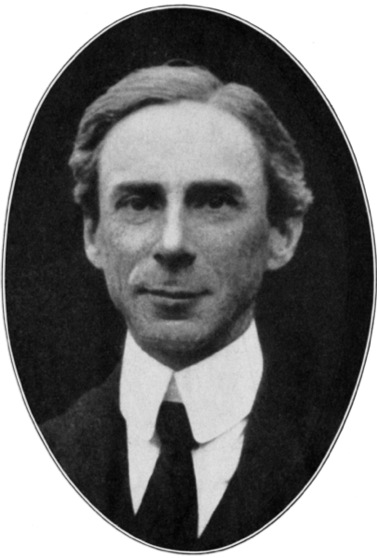
\includegraphics[scale=0.5]{img/Russell.eps}
 \captionsetup{labelformat=empty}
 \caption{伯特兰$\cdot$罗素 1872-1970}
 \label{fig:Russell}
\end{wrapfigure}

%Monmouthshire
\index{罗素}
罗素1872年生于英国蒙茅茨郡的一个贵族家庭。两岁时母亲去世,三岁时父亲也去世。6岁时祖父也去世了,于是罗素和祖母生活在一起。祖母对他的童年和青少年时期的发展有过决定性的影响。她曾告诫罗素:“你不应该追随众人去做坏事”,罗素一生都努力遵循这条准则。

罗素少年时代未被送到学校去学习,而是在家接受教育。1883年开始,11岁的罗素跟随堂哥弗兰克学欧几里德几何。不久,罗素开始接触哲学思辨,并在宗教问题上,悄悄写下自己的想法在一家杂志发表。1890年罗素考入剑桥大学三一学院,大学前三年,他专攻数学,获数学荣誉学位考试的第七名。1894年,参加伦理学荣誉学位考试。完成研究论文《论几何学的基础》。在剑桥期间,他结识了当时的数学讲师怀特海等人。1895年,罗素在三一学院获得了研究员的职位。二十世纪初,他发现了著名的罗素悖论,并引发了一场关于数学基础的大讨论。其后十多年间,罗素投身于数学基础和数理逻辑的研究中。1920年,罗素应邀到中国讲学一年。足迹遍及中华南北,作了多场演讲。话题从数理逻辑到切中时弊的社会改造建议,在当时成为中国文化界的一件盛事。给我国哲学界以很大的影响。他的《西方哲学史》在我国的哲学爱好者中有着广泛的影响。

二十世纪50年代后,罗素从哲学转向国际政治。他反对核战争、主张核裁军。由于伸张民主和参加核裁军运动,罗素一生曾两次被捕入狱。其中第二次入狱时已经是89岁高龄。1950年罗素获得诺贝尔文学奖。委员会在授奖时称他为“当代理性和人道的最杰出代言人之一,西方自由言论和自由思想的无谓斗士。”

1970年2月2日,罗素在彭林德拉耶斯逝世,他的骨灰被撒在威尔士的群山之中。
% Russell died of influenza on 2 February 1970 at his home in Penrhyndeudraeth. His body was cremated in Colwyn Bay on 5 February 1970. In accordance with his will, there was no religious ceremony; his ashes were scattered over the Welsh mountains later that year.

\subsection{罗素悖论的影响}

罗素发现集合论基础的悖论后极为沮丧。他后来回忆道:“每天早晨,我面对一张白纸坐在那儿,除了短暂的午餐,我一整天都盯着那张白纸。常常在夜幕降临之际,仍是一片空白……似乎我整个余生很可能就消耗在这张白纸上。让人更烦恼的是,矛盾是平凡的。我的时间都花在这些似乎不值得考虑的事情上。”(\cite{HanXueTao16},第231页)罗素把他的发现告诉了数学家、逻辑学家弗雷格。当时弗雷格正在进行算术基础的建立工作,他的著作《算术的基本规律》已在付印中。弗雷格看到罗素悖论后非常沮丧,他写道:“一个科学家所遇到的最不合心意的事莫过于在他工作即将结束时,其基础崩溃了。罗素先生的一封信正好把我置于这个境地。”戴徳金也推迟了《什么是数的本质》一书的再版。罗素悖论涉及的是集合论中最基础的部分。由于集合论逐渐被大家接受,并进入了大多数数学分支,这使得人们对于数学和逻辑学的基本原理和有效性产生了怀疑。

\begin{Exercise}
\Question{我们可以用语言定义数,例如“最大的两位数”定义了99。定义一个集合,是所有不能用20个以内的字描述的数字。考虑这样一个元素:“不能用20个以内的字描述的最小数”,它是否属于这个集合?}
\Question{“这个世界上唯一不变的是变化”——这句话是否是罗素悖论?}
\Question{本章开头苏格拉底的话是否是罗素悖论?}
\end{Exercise}

\section{数学基础的分歧}

为了解决罗素悖论这一影响理性思维基础的问题,数学家们从1900年到1930年间持续进行讨论并各自提出了解决方案。数学在历史上长期被当作理性思维的真理,其绝对性和唯一性从未被引起怀疑和争论。在这一大讨论中,人们终于意识到,在不同的哲学观念下,可以存在不同的数学。

\subsection{逻辑主义}

\begin{wrapfigure}{L}{0.3\textwidth}
 \centering
 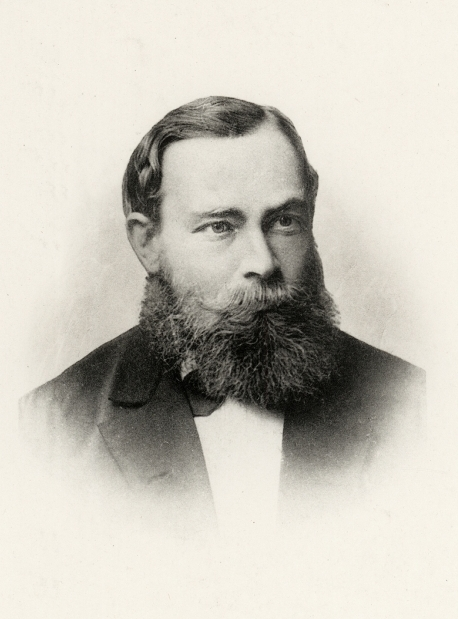
\includegraphics[scale=0.9]{img/Frege.eps}
 \captionsetup{labelformat=empty}
 \caption{戈特洛布$\cdot$弗雷格(1848-1925)}
 \label{fig:Frege}
\end{wrapfigure}

\index{弗雷格}
逻辑主义的早期代表人物是弗雷格。他认为数学的基础并不是数,算术理论可以建立在逻辑的基础上。弗雷格把朴素集合论看作是逻辑的一部分。他做的第一件工作是利用逻辑来定义自然数。我们知道数具有抽象的含义。3可以代表3个人、三个鸡蛋、图形中的三角等等,这些类\footnote{弗雷格的工作在康托尔之前,他当时使用了“类”(class)一词。康托尔后来使用了德语中的“集合”。}都有三个元素,用哪一个来代表自然数3呢?弗雷格的意见是:全部。即所有能和上述类一一对应的类所组成的,无穷的,抽象的类来定义自然数3。弗雷格的这一定义看起来有些复杂,但是很了不起。它突破了文化背景的限制。不管你是使用何种语言,何种符号,按照弗雷格的方法,对数字3的理解都不会有歧义。因为佛雷格的定义中根本不需要任何符号。这样佛雷格就定义了数——它是所有类的类。接下来佛雷格借助这一定义和逻辑理论建立了自然数的理论,进而形成了逻辑化的算术理论。再进一步,弗雷格打算从利用逻辑发展出除几何以外的全部数学。这就是他在《算术的基本规律》一书中打算完成的事情。由于弗雷格坚信逻辑的原则是完全可靠的,这样他的工作一旦完成,数学“就被固定在一个永恒的基础上了。”

我们知道接下来发生了什么。在《算术的基本规律》正在付印时,罗素的信“及时”寄到了。罗素悖论让弗雷格陷入了困惑。他工作的基础——利用逻辑定义数的概念——恰好是关于所有类的类。这样的定义直接导致了悖论的出现。弗雷格动摇了,并最终放弃了他的逻辑主义立场。

罗素接过了逻辑主义的火炬,积极投身于数学基础的重建和悖论的解决工作中。罗素坚信数学就是逻辑,逻辑就是数学。他形成这样的思想,意大利数学家皮亚诺起到了重要的作用。罗素后来回忆道:“在我学术生命中最重要的一年是1900年,而这一年中最重要的事是我去巴黎参加国际哲学会议……皮亚诺和他的学生们在一切讨论中所表现出来的,为他人所没有的精确性,给了我深刻的印象。”他和怀特海两人每天讨论数学的基本概念,经过艰苦的工作终于写出了著名的《数学原理》\footnote{罗素和怀特海希望通过书的名字向牛顿致敬。因为牛顿的著作名为《自然哲学中的数学原理》}三卷本分别在1910年到1913年间出版。这可以说是数理逻辑的经典之作。为了解决悖论,罗素指出一切悖论都源于某种“恶性循环”,而恶性循环源于某种不合法的集体,具体的说就是集体的整体这一概念。所以要想消除悖论、避免恶性循环,凡是涉及一个集体的整体的对象,它本身不能是该集体的成员。从这一思想出发,罗素提出了“分支类型论”。

\begin{wrapfigure}{R}{0.4\textwidth}
 \centering
 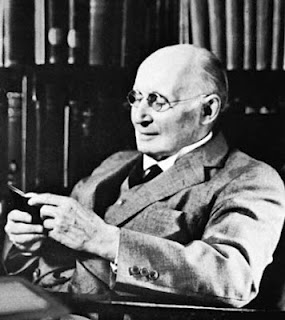
\includegraphics[scale=0.4]{img/Whitehead.eps}
 \captionsetup{labelformat=empty}
 \caption{阿尔弗雷德$\cdot$怀特海(1861-1947)}
 \label{fig:Whitehead}
\end{wrapfigure}

\index{分支类型论}
分支类型论将集合进行了层次划分,定义域中的对象个体属于第0类;个体的集合属于第1类;第1类中的个体的集合,也就是集合的集合,属于第2类……每一集合都必须从属确定的类。而命题中的对象必须从属于它所在的等级。这样做可以有效地消除悖论,但使用起来极其繁琐不便。《数学原理》第一卷直到第363页才推出数字1的定义。庞加莱挖苦道:“这是一个可亲可佩的定义,它献给那些从来不知道1的人。”使用分支类型论,所有的工作只能在各自的等级上进行,整数在整数的等级上,有理数在有理数的等级上,我们不能把$n/1$和$n$混为一谈。更为严重的是:“所有实数……”这样的命题不合法了,因为它涉及了集合中不同的层次。

\index{约化公理}
但最有争议的地方是“无穷公理”、“选择公理”、“约化公理”的使用。为了处理自然数以及更为复杂的实数和超限数,罗素和怀特海引入公理来承认无穷的存在。他们也承认可以从非空集合,甚至无穷集合中选择元素组成新的集合。这两条有争议的公理在集合论中也存在,但最难以让其他数学家接受的是约化公理。为了支持数学归纳法,约化公理认为任何较高层次的一个命题与一个层次为0的命题等价。约化公理激起了反对,因为它显得太任意了。1909年庞加莱说:约化公理比数学归纳法更靠不住,更含糊不清。

后来连罗素自己也动摇了:“从严格的逻辑化来看,我找不出任何理由来相信约化公理是逻辑必然的,这就是说,它在所有可能的世界中都是真的。因此,在逻辑体系中,承认这个公理是个缺憾,即使从经验来看是真的。”\cite{M-Kline-2007}

\subsection{直觉主义}

\begin{wrapfigure}{L}{0.4\textwidth}
 \centering
 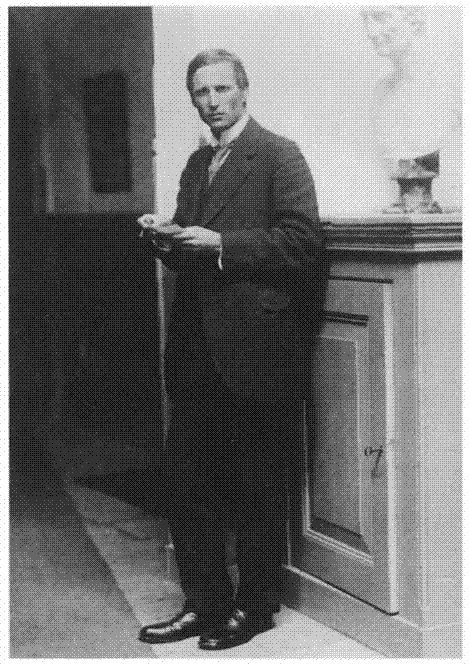
\includegraphics[scale=0.28]{img/Brouwer.eps}
 \captionsetup{labelformat=empty}
 \caption{布劳威尔(1881-1966)}
 \label{fig:Brouwer}
\end{wrapfigure}

%图片来自The Low Countries, Arts and Society in Flanders and the netherlands. A year book 1998-99
\index{布劳威尔}
与逻辑主义同时,另一群称为直觉主义的数学家使用了截然不同、完全相反的方法来重建数学的基础。直觉主义可以追溯到帕斯卡,其先驱是上一章介绍的过的德国数学家克罗内克。鲍莱尔、勒贝格、庞加莱、外尔等一批数学巨匠都是直觉主义的支持者。其代表人物是荷兰数学家布劳威尔。布劳威尔于1881年生于荷兰鹿特丹附近的小镇奥弗希。1897年他考入阿姆斯特丹大学攻读数学。在读大学时,他获得了关于四维空间连续运动的某些结果,并发表在阿姆斯特丹皇家科学院报告集上。在当大学生时,通过自己的刻苦钻研,更由于受到曼诺利(Mannoury)教授一系列启迪性讲座的启发,布劳威尔接触到了拓扑学和数学基础,并且终生钟爱它们。

受到希尔伯特在巴黎的第二届国际数学家大会的讲演的影响,布劳威尔从1907年到1913年进行了大量拓扑学的研究。建立布劳威尔不动点定理是他的突出贡献。这个定理表明:在二维球面上,任意映到自身的一一连续映射,必定至少有一个点是不变的。他把这一定理推广到高维球面。尤其是在$n$维球内映到自身的任意连续映射至少有一个不动点。1910年,布劳威尔证明了维数的拓扑不变性。1913年,他给出了拓扑空间维数的严格定义。由于布劳威尔在拓扑学上的出色成就,他被推选为荷兰皇家科学院院士。

在攻读博士学位时,布劳威尔以极大的热情关注着罗素和庞加莱关于数学的逻辑基础的论战\footnote{庞加莱认为逻辑和直觉是数学与科学中不可或缺的两个重要方面。逻辑可以帮助我们严密化,直觉是发明和创造所必须的。逻辑不能完全替代直觉。直觉可能导致假象\cite{Poincare2}。},并以此为题写成他的博士论文。总的说来,他倾向于庞加莱的观点,反对罗素和希尔伯特关于数学基础的思想。但是,他又不同意庞加莱关于数学存在性的说法。他认为,庞加莱的办法不能排除悖论。为此,他在博士论文“论数学基础”中开始建立直觉主义的数学哲学。1966年,85岁的布劳威尔不幸死于车祸。

布劳威尔的直觉主义来源于他的哲学。数学是起源和产生于头脑的人类活动,它并不存在于头脑之外,因此,它是独立于真实世界的。头脑识别基本的、清晰的直觉,这些直觉不是感觉或经验上的,而是对某些数学概念直接的确定,其中包括整数。布劳威尔认为数学思维是智力构造的一个过程,它建造自己的天地,独立于经验,并且只受到必须建立于基本的数学直觉之上的限制。这种基本的直觉概念不应被理解为像在公理理论中的那种未定义概念,而应设想为某种东西,只要它们在数学思维中确实是有用的,用它就可以对出现在各种数学系统中的未定义概念做出直观上的理解。

\begin{wrapfigure}{R}{0.3\textwidth}
 \centering
 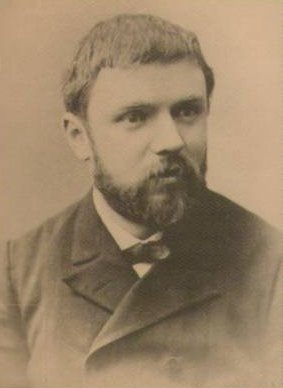
\includegraphics[scale=0.4]{img/Poincare.eps}
 \captionsetup{labelformat=empty}
 \caption{庞加莱(1854-1912)}
 \label{fig:Poincare}
\end{wrapfigure}

布劳威尔认为“要在这个构造过程中发现数学唯一可能的基础,必须再三思考,反复斟酌。哪些论点是直觉上可接受的,头脑中所自明的;哪些不是。”是直觉而不是经验或逻辑决定了概念的正确和可接受性。当然,这一陈述并未否认经验所起的历史作用。除了自然数以外,布劳威尔坚持认为加法、乘法和数学归纳法在直觉上是清晰的。而且,当头脑已获得自然数1,2,3……的概念后,使用“空洞形式”无限重复的可能性,从$n$到$n+1$的步骤,就产生了无穷集合。然而,这种集合只是潜无穷,因为对于任一给定的有限数集,总可以加入一个更大的数。布劳维否定了康托尔的所有元素都“一下子”出现的无限集,并因此否定了超限数理论、策梅罗的选择公理以及使用了真正的无限集的那部分分析。在1912年的一次演讲中,布劳威尔甚至接受了直至$\omega$的基数和可数集。

布劳威尔坚持要求可构造性,否定无限制地使用排中律,尤其在涉及无穷时。这样一来传统数学中的许多内容都必须被丢弃了。例如欧几里得关于素数有无穷多的证明,并没有依次构造出素数,而是通过排中律指出存在性。这样在直觉主义看来是不可接受的。为了让其他数学家信服,1924年,布劳威尔提出了扇形定理。这一定理表明存在这样的性质,对于有界展延的全部元素来说,可以使它要么持有这种性质要么不持有这种性质。对排中律的否定产生了一种新的可能性——不可判定的命题。对于无穷集合,直觉主义主张还有第三种状况,即可以有这样的命题,既不是可以证明的,也不是不可以证明的。

总体来说直觉主义在当时的工作中批判多于建设。直觉主义否定了一大批数学成果。包括无理数概念,函数论、康托尔的超限数。一大批推理模式包括排中律都无法使用。因此遭到了其他数学家们的强烈反对,希尔伯特说:“与现代数学的浩翰大海相比,那点可怜的残余算什么。直觉主义者所得到的是一些不完整的、没有联系的孤立的结论。”

%第二次世界大战后,由于克里尼(Kleene)开拓性的研究、递归函数论的兴起和计算机的广泛发展,使得直觉主义的基础复活了,它被更多的数学家所接受。

\subsection{形式主义}

\begin{wrapfigure}{L}{0.5\textwidth}
 \centering
 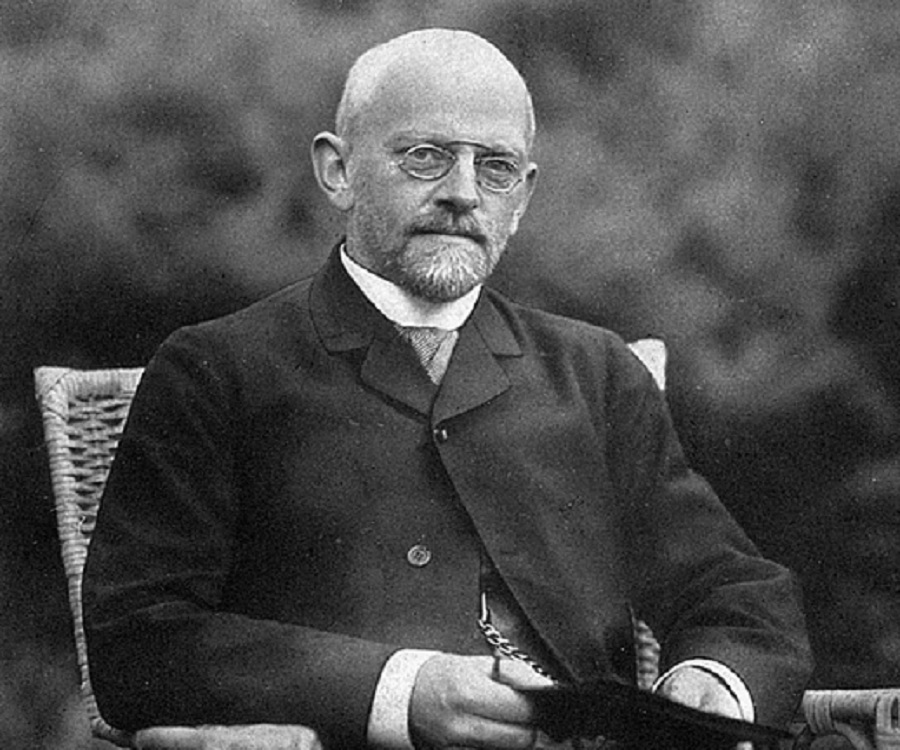
\includegraphics[scale=0.25]{img/Hilbert.eps}
 \captionsetup{labelformat=empty}
 \caption{大卫$\cdot$希尔伯特(1862-1943)}
 \label{fig:Hilbert}
\end{wrapfigure}

\index{希尔伯特}
关于数学基础思想的第三大派系是由希尔伯特领导并风行一时的形式主义流派。希尔伯特是伟大的德国数学家,1862年生于东普鲁士的哥尼斯堡。他从小勤奋好学,对于科学特别是数学表现出浓厚的兴趣。1880年,希尔伯特进入哥尼斯堡大学学习数学。在这里结识了比他年长三岁的副教授胡尔维茨和比他高一班的闵可夫斯基。希尔伯特后来这样追忆他们的友谊:“在日复一日无数的散步时刻,我们漫游了数学和科学的每个角落。”

% 一边散步一边谈论数学成为他特有的风格。有一则与之有关的趣事。希尔伯特日复一日地穿着一条破裤子,人们看到了都觉得尴尬。把这种情况得体地告诉希尔伯特落到了他的助手,数学家柯朗的身上。柯朗知道希尔伯特喜欢一边谈论数学,一边在乡间漫步。于是便邀请他一同散步。柯朗故意带着希尔伯特走过一片长着刺的灌木丛,然后告诉他裤子被刮破了。“哦,不是。”希尔伯特回答说:“它几个星期前就是这样了,不过还没有人注意到。”

1895年,数学领袖克莱因邀请希尔伯特去哥廷根大学。希尔伯特在那里渡过了48年直到去世。他与克莱因一起,开创了哥廷根学派的全盛时期,把哥廷根大学变成了全世界的数学中心。世界各地的学生把哥廷根看作数学的圣地:“打起背包,到哥廷根去!”

希尔伯特是二十世纪前后最伟大的数学家之一。当时唯一可以与其并驾齐驱的是法国数学家庞加莱。他在数学几乎所有领域都作出了巨大贡献。以希尔伯特命名的数学名词多如牛毛,有些连希尔伯特本人都不知道。比如有一次,希尔伯特问系里的同事“请问什么叫做希尔伯特空间?”。他去世时,美国的《自然》杂志上写道:“希尔伯特就像数学世界的亚历山大,在整个数学版图上,都留下了他那巨大显赫的名字。”\cite{HanXueTao16}

1900年,在巴黎召开的第二届国际数学家大会上,希尔伯特提出了新世纪数学家应当努力解决的23个数学问题,被认为是20世纪数学的至高点,对这些问题的研究有力推动了20世纪数学的发展,在世界上产生了深远的影响。

希尔伯特帮助培养了一大批顶级的数学家,包括外尔、柯朗、埃米$\cdot$诺特、冯$\cdot$诺伊曼、策梅罗等等。1933年纳粹上台,驱赶了大批犹太裔师生。1943年,希尔伯特在孤独中逝世。在他的墓碑上,留下了他那极富感染力的乐观主义名言:“我们必须知道,我们必将知道。”

希尔伯特的《几何基础》(1899)是公理化思想的代表作,书中把欧几里得几何学加以整理,成为建立在一组简单公理基础上的纯粹演绎系统,并开始探讨公理之间的相互关系与研究整个演绎系统的逻辑结构。1904年,希尔伯特开始着手研究数学基础问题,经过多年酝酿,于二十年代初,提出了如何论证数论、集合论或数学分析一致性的方案。他建议从若干形式公理出发将数学形式化为符号语言系统,并从不假定实无穷的有穷观点出发,建立相应的逻辑系统。然后再研究这个形式语言系统的逻辑性质,从而创立了元数学和证明论。希尔伯特的目的是试图对某一形式语言系统的无矛盾性给出绝对的证明,以便克服悖论引起的危机,一劳永逸地消除对数学基础以及数学推理方法可靠性的怀疑。

为了实现这一主张,希尔伯特规划了他的方案,主要内容是:
\begin{enumerate}
\item 证明古典数学的每个分支都可在数学系统公理化意义下予以公理化。
\item 证明每一个在上述意义下被公理化了的系统都是完备的。即系统内任一可表述的命题均可在系统内得到判定。
\item 证明每一个在上述意义下的系统都是相容的。
\item 证明每个这样的系统所相应的模型都是同构的。
\item 寻找这样一种方法,借助于它,可在有限步骤内判定任一命题的可证明性。
\end{enumerate}

希尔伯特为具体实施其规划而创立证明论,即元数学理论。它着眼于整个形式系统,并以“证明”本身作为研究对象。这样就区分出三种数学系统:
\begin{enumerate}
\item 非形式化的数学系统$G$:即普通的数学系统,在其中允许使用古典逻辑推理规则,例如,在无穷集合上使用排中律等。
\item 形式化的数学系统$H$:在$H$中的符号、公式、公理、命题等都是形式的,在未加解释之前都是没有内容和意义的,而经解释后就是$G$中相应的内容。即$G$是$H$的模型,$H$是$G$的形式化。用希尔伯特的一句名言来举例:“我们必定可以用‘桌子、椅子、啤酒杯’来代替(几何中的)‘点、线、面’。”在这种处理下,原几何理论中所包含的特定意义和直观背景被完全舍弃。我们研究的只是未定义项之间的关系,而关系由公理组来体现。
\item 元数学系统$K$:这是用以研究$H$的元理论,而在$K$中的推理规则必须保持直觉的可信性,例如不能涉及无穷,不允许在无穷集合上使用排中律等。
\end{enumerate}

就在希尔伯特实施他的规划时,1931年,年轻的哥德尔发现了不完全性定理,从本质上宣告了希尔伯特计划是行不通的。我们将在后面详细介绍这一发现。

\subsection{公理集合论}

与逻辑主义、直觉主义、形式主义不同,集合论公理化派的成员在开始时并没有形成他们独特的哲学,但是他们逐渐获得了支持,有了明确的方案。在今天,我们可以肯定地说这个派别在数学家中所拥有的支持者是与我们前面介绍的三个派别势均力敌的。

集合论公理化的起源可以追溯到戴德金和康托尔的工作中。尽管他们主要关心的是无穷集合问题,并且也都着手于在集合概念的基础上建立整数的概念。一旦整数建立了,也就能推导出全部数学了。当罗素悖论和集合论的矛盾出现时,一些数学家相信这是由于滥用集合所致。康托尔的集合论的整个表示形式在今天通常被说成“朴素集合论”。因此集合论的公理化思想,做为一种经仔细选择的公理化基础,可以排除集合论中的悖论,正如几何和数系中的公理化可以在那些领域里解决逻辑问题一样。1908年数学家策梅罗沿着这一方向进行了一次成功的尝试。

\index{策梅罗}
策梅罗希望清晰明确的公理能够澄清集合的含义和集合所应具有的属性,尤其是他想要设法限制集合的大小。他没有什么哲学根据,只是力图避免矛盾。他的公理系统包含未加定义的集合的基本概念,以及一个集合被另一个集合所包含的关系。所有这些加上已定义的概念就可以满足公理中的陈述,只有公理所提供的集合的性质才能使用。在公理中,无穷集的存在性,以及像集合的并与子集的形成这一类的运算也由公理给出。策梅罗也用到了选择公理。

\begin{figure}[htbp]
  \centering
  \subcaptionbox{恩斯特$\cdot$策梅罗(1871-1953)}[0.45\linewidth]{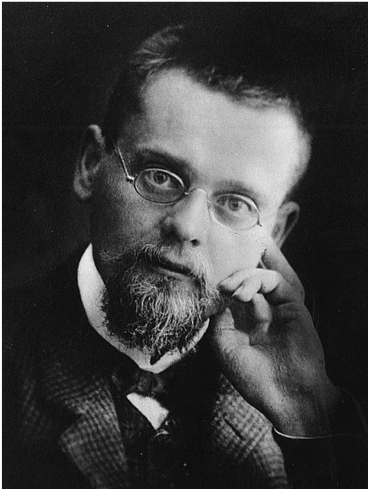
\includegraphics[scale=0.7]{img/Zermelo.eps}} \quad
  \subcaptionbox{亚伯拉罕$\cdot$弗兰克尔(1891-1965)}[0.45\linewidth]{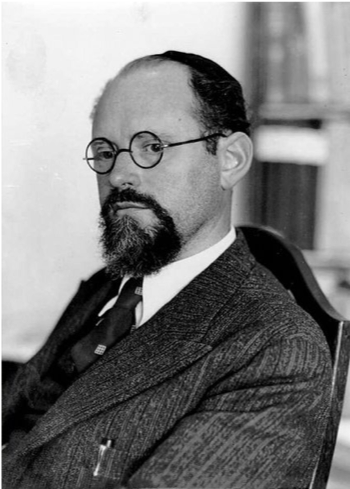
\includegraphics[scale=0.7]{img/Fraenkel.eps}}
  \captionsetup{labelformat=empty}
  \caption{}
  \label{fig:Zermelo-and-Fraenkel}
\end{figure}

\index{ZF系统} \index{弗兰克尔}
策梅罗的公理系统在1922年由弗兰克尔改进。策梅罗没有区分集合的属性和集合本身,它们被当作同义语使用。弗兰克尔在1922年找出了它们之间的区别。这套被集合论公理化者最通常使用的公理系统叫做策梅罗-弗兰克尔系统,简称ZF系统。他们俩分别预测到了精致的、严密的数学逻辑的可行性,却没有详细说明逻辑的原理。他们认为这些都是在数学范围之外的,并且确信他们可以像1900年以前的数学家使用逻辑一样来使用这些逻辑原理。

策梅罗在1908年的论文中给出了集合论的7条公理。1930年又加入了弗兰克尔、斯克朗、冯$\cdot$诺伊曼建议的两条公理。这些公理表示如下:

\index{选择公理}
\begin{enumerate}
\item \textbf{外延公理}:如果两个集合含有相同的元素,那么它们相等。形式化就是对于集合$A$和$B$,若$A \subseteq B$且$B \subseteq A$,则$A = B$。外延公理相当于逻辑上的同一律。
\item \textbf{空集}:空集存在。
\item \textbf{分离公理}:任何可用理论形式化的属性都可以用来定义一个集合。即对集合$S$,命题函数$p(x)$是确定的,则存在集合$T = \{ x | x \in S, p(x)\}$。分离公理也称作概括公理。
\item \textbf{幂集公理}:对任一集合,都可以作出其幂集;即任一给定集合中的所有子集的全体也是一个集合(这个过程可以无限次重复)。
\item \textbf{并集公理}:一组集合的并也是一个集合。
\item \textbf{选择公理}:设$S$为一个由非空集合所组成的集合,可以从每一个在$S$中的集合中,都选择一个元素和其所在的集合配成有序对来组成一个新的集合。选择公理简称为AC。
\item \textbf{无穷公理}:存在一集合$Z$,它含有空集,对任一对象,若$a \in Z$,则$\{a\} \in Z$。(这一公理保证了无限集是可构造的。)
\item \textbf{替换公理}:这条公理是弗兰克尔1922年引入的。对于任意的函数$f(x)$和集合$T$,当$x \in T$时,$f(x)$都有定义的前提下,一定存在一集合$S$,对于所有的$x \in T$,在集合$S$中都有一元素$y$,使$y = f(x)$。也就是说,由$f(x)$定义的函数其定义域在$T$中的时候,它的值域可限定在$S$中。
\item \textbf{正则公理}:这条公理是冯$\cdot$诺伊曼1925年引入的。$x$不属于$x$。
\end{enumerate}

这样,集合论就被抽象成一个公理化的理论。集合成了未定义概念,它是满足上述公理的对象。通过这样的限制,避免了“所有对象”这样的说法,从而避免了悖论,弥补了朴素集合论的缺陷。但是就这些公理的选择和承认仍然存在争议。其中最大的争议来自选择公理。

%\begin{wrapfigure}{R}{0.5\textwidth}
\begin{figure}[htbp]
 \centering
 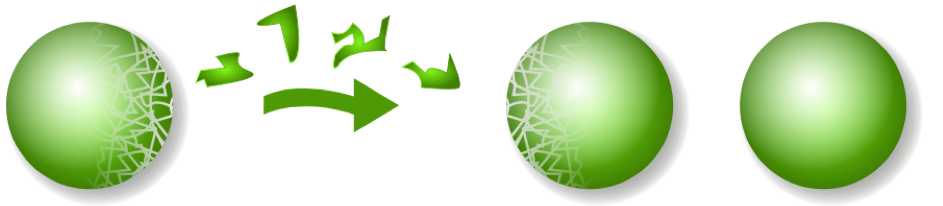
\includegraphics[scale=0.6]{img/Banach-Tarski-Paradox.eps}
 %\captionsetup{labelformat=empty}
 \caption{巴拿赫-塔斯基“悖论”:一个球可以分解和重新组合成两个大小和原来一样的球}
 \label{fig:Banach-Tarski-Paradox}
\end{figure}
%\end{wrapfigure}

\index{分球定理} \index{ZFC系统}
1924年波兰数学家巴拿赫和塔斯基证明了分球定理\footnote{又称为豪斯多夫-巴拿赫-塔斯基定理,或者“分球怪论”}。这一定理指出在选择公理成立的情况下,可以将一个三维实心球分成有限(不可测的)部分,然后仅仅通过旋转和平移到其他地方重新组合,就可以组成两个半径和原来相同的完整的球。巴拿赫和塔斯基提出这一定理原意是想拒绝选择公理,但该证明很自然,因此数学家认为这仅意味着选择公理可以导致少数令人惊讶和反直觉的结果,有人提出不应该把它包含进来。不包含选择公理的集合论被称为ZF系统,包含选择公理的被称为ZFC系统。我么在上一章曾介绍过选择公理和连续统假设之间的有趣关系。

\section{哥德尔不完全性定理}

这样,到1930年,四种彼此独立的、截然不同的并且或多或少有些冲突的关于数学基础的方法都已亮相。并且可以毫不夸张地说,他们彼此的追随者也都处于对峙状态。一个人再也不能说一条数学定理是被正确地证实了,因为到1930年,他必须加上一句,即依照谁的标准它被认为是正确的。除了直觉主义者认为人的直觉能保证相容性外,数学的相容性,这个激发了新方法的重要问题,根本就没有得到解决。希尔伯特还在乐观地规划着证明数学是完备的和一致的。改变这一切的是年轻的数学家、逻辑学家哥德尔。

\begin{wrapfigure}{L}{0.4\textwidth}
 \centering
 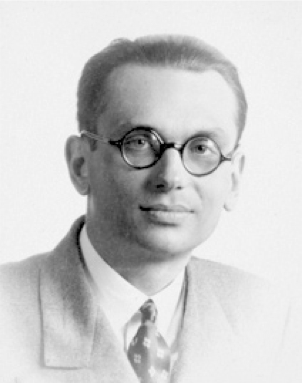
\includegraphics[scale=0.8]{img/Godel-young.eps}
 \captionsetup{labelformat=empty}
 \caption{库尔特$\cdot$哥德尔(1906-1978)}
 \label{fig:Godel-young}
\end{wrapfigure}

\index{哥德尔}
哥德尔于1906年生于奥匈帝国的布尔诺(今属捷克共和国)。8岁时突患急性风湿热,很可能是这次疾病的后果,哥德尔后来不断被妄想症困扰。童年时期他充满好奇心,被家里人叫作“为什么先生”。1924年哥德尔考入了维也纳大学学习物理。接触了数论的课程后,很快哥德尔意识到数学才是自己真正的追求。于是1926年转入数学系。哥德尔对于哲学也很有兴趣,经常参加哲学小组的讨论,旁听哲学教授的课程。对哲学的探索贯穿着哥德尔的一生。

1929年夏天,23岁的哥德尔证明了“狭谓词演算的有效公式皆可证”,并于1930年以此获得了博士学位。随后,他进一步研究希尔伯特规划,试图寻找在有限步骤内证明自然数系统的相容性和一致性的办法。但是哥德尔得到了一个意外的结果。1930年在哥尼斯堡召开的数学讨论会上,他公布了这一结果——即伟大的哥德尔第一不完全性定理。不久他又证明了第二不完全定理。

1933年后,哥德尔一直在维也纳大学工作。希特勒上台后,纳粹开始插手奥地利的学术界。1936年,维也纳学派的物理学家和逻辑学家摩里兹$\cdot$石里克被一个学生刺杀,当场死亡。哥德尔参加过石里克的讨论组,因此深受刺激,他患上了妄想症,总疑心有人要毒杀自己。二战爆发后,哥德尔接受了普林斯顿高等研究院的邀请来到美国。在这里他结识了爱因斯坦并成为了终身好友。他们经常一起在普林斯顿散步和闲谈。1955年爱因斯坦去世对哥德尔的情绪有很大打击。哥德尔晚年,美籍华裔逻辑学家王浩是他最好的朋友之一。

哥德尔的妻子阿黛尔(Adele Nimbursky)比他大六岁。哥德尔21岁两人认识时,阿黛尔已婚且在夜总会工作。他们的婚姻遭到哥德尔家人反对,但有情人终成眷属,在1938年9月20日结婚。哥德尔的晚年一直和妄想症斗争,他唯恐有人下毒,只吃妻子阿黛尔做的食物。1977年阿黛尔动手术住院后,他干脆什么都不吃了。1978年1月,“因营养不良和身体机能衰竭”与世长辞,死时体重只有60磅。由于在在逻辑方面的杰出贡献,人们把他视为自亚里士多德以来最伟大的逻辑学家。

\index{哥德尔不完全性定理}
1931年,哥德尔发表了论文“论《数学原理》及有关系统中的形式不可判定命题”,题目中的《数学原理》就是罗素和怀特海的巨著。哥德尔证明了在任何包含自然数算术的形式系统中,如果它是相容的,则必定存在一不可判定命题$G$,即不能证明$G$,也不能证明$G$的否定。这一定理被称为哥德尔第一不完全性定理。这一定理表明,无矛盾的形式化系统是不完全的。只要系统强大到足以包含自然数公理系统,都会有超越于它的问题。人们自然会想,既然$G$是不可判定的命题,如果把$G$或者$G$的否定作为公理加入到系统中,不就可以得到一个更为强大的系统了么?但是不久哥德尔进一步证明了第二不完全性定理。它表明,如果一个足以包含自然数算术的公理系统是无矛盾的,那么这种无矛盾性在该系统内是不可证明的。所以不论是把$G$或是$G$的否定当作公理加入系统,得到的新系统仍然是不完全的。总是存在更高一层的不可判定命题。

例如在欧几里得几何中,如果把第五公设抽出,仅仅使用前四条公理的形式化系统既不能证明第五公设,也不能证否第五公设。我们后来知道承认或者否定第五公设都会导致无矛盾的几何——分别是欧几里得几何和不同的非欧几何。再比如在公理集合论ZF系统中,既不能证明也不能证否选择公理,承认选择公理得到无矛盾的ZFC系统,而否定选择公理得到另一无矛盾的系统。即使加入选择公理,在ZFC中既不能证明也不能证否连续统假设。承认连续统假设得到一种无矛盾的系统,否认连续统假设得到另外的无矛盾系统。

%\begin{wrapfigure}{R}{0.5\textwidth}
\begin{figure}[htbp]
 \centering
 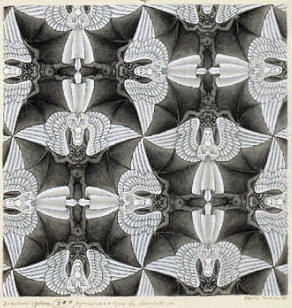
\includegraphics[scale=1]{img/Angel-Devil-1941.eps}
 %\captionsetup{labelformat=empty}
 \caption{埃舍尔《天使与魔鬼》1941}
 \label{fig:Angel-Devil-1941}
\end{figure}
%\end{wrapfigure}

哥德尔第一不完全性定理和第二不完全性定理合称为“哥德尔不完全性定理”。这等于宣布了希尔伯特纲领是行不通的。即便基本算术系统是协调的,那么这种协调性也不可能在算术系统内证明。伟大的数学家安德烈$\cdot$韦伊评论说:“因为数学具有一致性,所以上帝与我们同在;因为我们不能证明这一点,所以魔鬼亦与我们同在。”\cite{HanXueTao16}

\section{不完全性定理的证明}

按照希尔伯特规划,首先是把整个数学理论组织成一个形式系统。然后在元数学中对这一形式系统进行研究。为此我们需要把古典数学的每一分支表述为这样的形式系统。其中只包含有限条公理,然后通过元数学证明这样的系统是完备的且无矛盾的。其中最基本的一个系统就是自然数算术,因为很多数学系统都同构于它。在上一章,我们看到了如何从自然数出发定义出整数,有理数,甚至实数。从实数对应到点,我们又可以利用解析几何把欧几里得几何算术化。

\subsection{构建形式系统}
\index{TNT系统} \index{印符数论}
这里我们采用侯世达在《哥德尔,埃舍尔,巴赫——集异璧之大成》中的方法和术语来简要介绍这一证明过程。哥德尔不完全性定理的证明也是从构建形式系统开始的。我们称这一系统为“印符数论”简称TNT\footnote{印符数论的英文Typographical Number Theory首字母的缩写。}。恰巧这也是黄色炸药三硝基甲苯的分子式,暗示其威力大到足以——摧毁自己这座大厦。所谓印符数论,就是把用我们熟悉的自然语言表示的数论形式化为一系列印刷字符。这看起来很复杂,但是在我们第一章中介绍的皮亚诺公理的基础上,其实并不难。首先我们要定义数字,按照皮亚诺公理,零是自然数,每个自然数都有其后继,我们很自然地可以这样定义数的印符:

\vspace{5mm}
\begin{tabular}{|r|l|}
零 & 0 \\
\hline
一 & S0 \\
\hline
二 & SS0 \\
\hline
三 & SSS0 \\
\hline
…… & …… \\
\end{tabular}
\vspace{5mm}

其中符号S代表后继,两个S表示后继的后继。一百个S和一个0表示0的一百次后继,也就是自然数100。尽管很长,但是规则异常的简单。定义了自然数,我们还要定义变量,为了是系统尽量简单,我们可以仅使用5个印符字母$a, b, c, d, e$。当需要更多变量时我们就加撇号,$a', a'', a'''$。接下来我们需要加法符号“$+$”和乘法符号“$\cdot$”以及辅助运算顺序的左右括弧。为了形式化命题我们需要等号“$=$”,表示否定的$\lnot$,表示蕴含的箭头$\to$。这样我们就可以表示命题了,例如(先不论命题的真假):

\begin{itemize}
\item 一加二等于四:$(S0 + SS0) = SSSS0$
\item 二加二不等于五:$\lnot (SS0 + SS0) = SSSSS0$
\item 如果1等于0,那么0等于1:$(S0 = 0) \to (0 = S0)$
\end{itemize}

一个命题中可以含有自由变元,例如:

\[
(a + SS0) = SSS0
\]

表示$a$加上2等于3。显然$a$的取值决定这个命题的真假,为此我们还需要引入存在量词符号$\exists$和全称量词符号$\forall$,以及表示量词约束关系的的冒号“:”。这样命题:

\[
\exists a : (a + SS0) = SSS0
\]

就表示:存在$a$使得$a$加上2等于3。再看另一个例子:

\[
\forall a : \forall b : (a + b) = (b + a)
\]

这恰好就是自然数的加法交换律。如果去掉$a$的量词约束,就变成:

\[
\forall b : (a + b) = (b + a)
\]

这是一个开公式,其中$a$是自由变元。它表示未指定的$a$可以与$b$交换。当然这一命题的真假并没有确定。为了把命题复合起来,我们还需要析取符号$\land$,合取符号$\lor$。尽管TNT中的符号极少,可是它的表达能力却很强,我们举一些例子看:

2不是任何数的平方:$\lnot \exists a : (a \cdot a) = SS0$

费马大定理在$n$为3时成立:$\lnot \exists a : \exists b : \exists c : ((a \cdot a) \cdot a) + ((b \cdot b) \cdot b) = ((c \cdot c) \cdot c)$

现在,我们只是有了可以表示命题的印符,为了构建TNT形式系统,我们还需要公理和推理规则。

\subsubsection{公理和推理规则}

仿照皮亚诺算术的公理,我们为TNT系统定义下述的公理:

\begin{enumerate}
\item $\forall a : \lnot Sa = 0$,这条公理说,没有任何自然数的后继是零;
\item $\forall a: (a + 0) = 0$,这条公理表示任何数加零都等于它本身;
\item $\forall a: \forall b: (a + Sb) = S(a + b)$,这条公理定义出了自然数的加法;
\item $\forall a: (a \cdot 0) = 0$,这条公理表示任何自然数乘以零都为零;
\item $\forall a: \forall b: (a \cdot Sb) = ((a \cdot b) + a)$,这条公理定义出自然数的乘法。
\end{enumerate}

接下来我们构建推理规则。比如我们希望从公理1,零不是任何自然数的后继这一普通情况,导出1不是零的后继这一特殊情况,为此我们需要引入特称规则:

\textbf{特称规则}:如果$u$是出现在印符串$x$中的变元。如果$\forall u: x$是一个定理,则$x$也是定理,并且对$x$中的$u$做任何替换得到的新印符串也是定理。

这里有一个限制,在替换$u$时,不能包含任何$x$中被量化的变元,并且替换要一致。与特称规则相反的是概括规则。这个规则允许我们把全称量词加到定理的前面。

\textbf{概括规则}:如果$x$是一个定理,其中的变元$u$是自由出现的。则$\forall u: x$也是一个定理。

例如,$\lnot S(c + S0) = 0$,表示不存在一个数加一的后继等于零,我们可以概括为:$\forall c: \lnot S(c + S0) = 0$。

接下来的规则可以让我们把全称量词和存在量词互换。

\textbf{互换规则}:如果$u$是一个变元,那么印符串$\forall u: \lnot $与$\lnot \exists u:$可互换。

例如公理1可以按照互换规则变成:$\lnot \exists a: Sa = 0$。接下来的一个规则允许我们在一个印符串的前面加上存在量词。

\textbf{存在规则}:假设一个项在定理中出现一次或多次,可以用一个变元来代替这个项,并且在前面加上存在量词。

我们还用公理1来举例:$\forall a: \lnot Sa = 0$中,我们可以把0,用变元$b$来代替,并且在前面加上存在量词。这样就得到:$\exists b: \forall a: \lnot Sa = b$。意思是说,存在一个数,使得任何自然数都不是它的后继。

接下来考虑相等的对称性和传递性,我们定义等号规则。令$r, s, t$都代表任意的项。

\textbf{等号规则}:
\begin{itemize}
\item 对称:如果$r = s$是定理,则$s = r$也是定理;
\item 传递:如果$r = s$和$s = t$都是定理,则$r = t$也是定理。
\end{itemize}

对于增、减后继符号$S$,我们也定义一个规则。

\textbf{后继规则}:
\begin{itemize}
\item 增加:如果$r = t$是定理,则$Sr = St$也是定理;
\item 去除:如果$Sr = St$是定理,则$r = t$也是定理。
\end{itemize}

现在的印符数论TNT已经很强大了,我们可以用它构造出各种比较复杂的定理。

\begin{Exercise}
\Question{尝试给出费马大定理的印符串。}
\Question{尝试用印符推理规则证明加法结合律。}
\end{Exercise}

\subsubsection{印符系统的不完全性}

使用TNT系统中的公理和推理规则不难证明下面的一系列定理:

\[
\begin{array}{rcl}
(0 + 0) & = & 0 \\
(0 + S0) & = & S0 \\
(0 + SS0) & = & SS0 \\
(0 + SSS0) & = & SSS0 \\
... & & ...
\end{array}
\]

第一条可以从公理2中,把$a$代换成0导出;第二条可以用公理3和上一条定理导出,每条定理都可以从上一条定理轻松导出。作为旁观者的我们,立刻想到这能不能概括成一条定理:

\[
\forall a: (0 + a) = a
\]

请注意它和公理2的区别。遗憾的是,利用迄今为止所给出的TNT规则,我们无法导出这一定理。我们也许希望添加一条规则,如果一系列这样的串都是定理,那么概括它们的全称量词串也是定理。但是这条规则只有在系统外部的人才能洞见。它不是一条可以放入形式系统的规则。

\index{omega不完全}
缺少这样的概括能力说明印符数论系统TNT是不完全的,确切地说,叫作$\omega$不完全的。这里的$\omega$恰恰就是上一章介绍的可数无穷基数。我们说一个系统是$\omega$不完全的,如果一系列无穷的串都是定理,而其全称概述却不是定理。并且更奇特地,这一印符串的否定形式:

\[
\lnot \forall a: (0 + a) = a
\]

也不是TNT中的定理。这意味着这个串在TNT中是不可判定的。这只是说TNT的能力不足以判定这个串是否是定理。就如同利用欧几里得几何的前四条公设无法判定第五公设一样。我们或者加入第五公设构成欧几里得几何;或者加入第五公设的否定构成非欧几何。我们可以将这一印符串或者其否定加入到TNT中,构造出不同的形式系统。

如果我们选择了这一印符串的否定,这里看似奇怪的一点是,零加上任何数都不再等于这个数了。这和我们通常熟悉的自然数加法大相径庭。但这恰恰提醒我们,所谓形式系统是带有未定义项的。我们只是方便理解选择了加号和自然数的含义。

印符系统TNT的$\omega$不完全性提示我们,我们的系统还缺少一条重要的规则——读者也许想到了——代表数学归纳法的皮亚诺第五公设。为此我们添上最后一块拼图。

\textbf{归纳规则}:如果$u$是印符串$X$中的一个变元,记为$X{u}$。如果把$u$替换为0时成立,且有$\forall u: X{u} \to X{Su}$。也就是若$u$时$X$成立,则将$u$替换为$Su$时$X$也成立。那么$\forall u: X{u}$是一个定理。

加上数学归纳法后,印符数论系统TNT终于和皮亚诺算术具有同样的能力了。

\begin{Exercise}
\Question{利用新加入的归纳规则证明$\forall a: (0 + a) = a$}
\end{Exercise}

\subsection{哥德尔配数}
\index{哥德尔配数}
哥德尔证明的最关键一步是引入了哥德尔配数。TNT系统已经强大到可以反映其它形式化系统,有没有可能利用TNT系统谈论它自身呢?哥德尔想到的办法就是把推理规则进行“算术化”。为此他把所有符号分配了一个数。

\begin{table}[htbp]
\centering
\begin{tabular}{|l|r||l|r|}
\hline
\textbf{符号} & \textbf{数} & \textbf{符号} & \textbf{数} \\
\hline
0 & 666 & S & 123 \\
\hline
= & 111 & + & 112 \\
\hline
$\cdot$ & 236 & ( & 362 \\
\hline
) & 323 & $a$ & 262 \\
\hline
$'$ & 163 & $\land$ & 161 \\
\hline
$\lor$ & 616 & $\to$ & 633 \\
\hline
$\lnot$ & 223 & $\exists$ & 333 \\
\hline
$\forall$ & 626 & : & 636 \\
\hline
\end{tabular}
\caption{对TNT系统进行哥德尔配数的一种方法}
\end{table}

这样公理1就可以做如下的翻译:

\begin{tabular}{cccccccc}
$\forall$ & $a$ & : & $\lnot$ & $S$ & $a$ & = & 0 \\
626 & 262 & 636 & 223 & 123 & 262 & 111 & 666 \\
\end{tabular}

配数的方法并不唯一。经过这样的配数,TNT中的任何串都可以表示为一个数了(尽管非常大)。现在问题来了,任给一个数,我们有没有办法判断它是一个TNT定理所代表的数呢?我们知道最开始有5个数一定是TNT数。它们就是五条公理所代表的数。根据TNT的推理规则,从这5个数开始,可以构造出无穷无尽的TNT数。在此之上我们引入一个数论谓词:

\begin{center}
$a$是个TNT数。
\end{center}

例如626,262,636,223,123,262,111,666是个TNT数(这里的逗号只是为了方便读写,和英文中每三位一分隔是同样的)它表示公理1。其否定形式是:

\begin{center}
$\lnot a$是个TNT数。
\end{center}

例如我们说123,666,111,666不是个TNT数。这意味着我们可以把$a$替换成0后面跟着123666111666个S。而这个巨大的串的含义实际是:$S0 = 0$不是TNT的定理。这意味着,TNT的确可以谈论它自己。这不是一种巧合,而是源于任何形式系统都可以在数论$N$中得到反映。于是我们形成了一个圈:形式系统TNT中的一个串有一个数论$N$中的解释,而$N$中的一个陈述可以有第二层含义,就是作为元语言对TNT的陈述。

\begin{figure}[htbp]
\centering
\begin{tikzpicture}[scale=0.8]
\draw (-5, 0) circle[x radius=1.5cm, y radius=1cm] node (TNT) {TNT}
      (0, 0) circle[x radius=1.5cm, y radius=1cm] node (N) {数论$N$}
      (5, 0) circle[x radius=1.5cm, y radius=1cm] node (Meta-TNT) {元TNT};
\draw[->] (TNT) to node [above] {数论解释} (N);
\draw[->] (N) to node [above] {元语言陈述} (Meta-TNT);
\end{tikzpicture}
\caption{TNT $\to$ 数论$N$ $\to$ 元TNT}
\label{fig:TNT-N-TNT}
\end{figure}

\subsection{构造自我指涉}

哥德尔做的最后一步是构造一个自我指涉。找到一个TNT串,称之为$G$,它是关于它自己的。其意义为:

\begin{center}
$G$不是TNT的定理
\end{center}

接下来我们可以引爆TNT了。那么究竟$G$是否是TNT中的定理呢?如果$G$是一个定理,那么它表示的就是真理,即:“G不是定理”。我们看到自指命题的威力了。由于充当了定理,$G$就不得不是个假理。根据我们的假定,TNT不会把假理当作定理,于是我们被迫得出结论说$G$不是个定理。但是知道了$G$不是个定理后,我们就得承认$G$表示了一个真理。这揭示出TNT没有达到我们的期望——我们发现了一个符号串,它表示了真理,然而却不是一个定理。但考虑$G$还有一个算术解释这一事实。它表示了关于自然数的某个算术性质的一个陈述。通过在TNT系统外面进行的推理,我们确定了这个陈述为真,还确定了这个串不是TNT的定理。我们问TNT这个串是否为真,TNT将既不能说“是”,也不能说“不”。

$G$就是那个不可判定命题。这就是哥德尔不完全定理的证明思路。

\section{万能的程序与对角线证明}
\index{原始递归函数}
哥德尔不完全性定理对于编程意味着什么呢?我们有一个在编程上完全同构的问题。为此,我们从设计一个形式化的计算机语言开始。这个语言支持原始递归函数。所谓原始递归函数是一类数论函数,它们可以从自然数映射到自然数,并遵循下面5条公理:

\begin{enumerate}
\item 常函数:0元常函数0是原始递归的;
\item 后继函数:一元后继函数$S(k) = k + 1$是原始递归的;
\item 投影函数:传入$n$个数,返回其中第$i$个数的函数$P_i^n$是原始递归的;
\item 组合:原始递归函数的有限次组合是原始递归的;
\item 原始递归:
\[
\begin{cases}
h(0) = k \\
h(n + 1) = g(n, h(n)) \\
\end{cases}
\]
称$h$是由$g$经原始递归运算得到的,可以扩展到多元的情况。
\end{enumerate}

包含加、减基本运算符号、条件分支(if-then)、等于、小于判断和有界循环的编程语言被称为原始递归的编程语言。所谓有界循环指循环的次数在进入循环体前是确定的。它可以是不带跳转语句(goto)的loop,或者是在循环体中不能改变循环变量的for循环。但不能是while循环或repeat-until循环。由于这些限制,所有原始递归的程序必然是确定停机的。

原始递归函数的一个重要性质是全部原始递归程序是递归可枚举的。假设我们可以从全部原始递归程序中筛选出那些只有一个输入一个输出程序,把它们列出,放入到一个无穷大的程序库里。我们给每个程序一个编号\footnote{其中一种编号方案是把程序文字的ASCII码连接起来形成一个数,然后把这些数从小到大排列。由于没有两个程序是相同的,所以其ASICII码形成的数也不同。},从自然数0开始,1,2,3……一直枚举下去。我们可以把这些程序记为$B[0], B[1], B[2], ...$。对于第$i$个程序,输入参数数$n$时得到结果是$B[i](n)$。

现在,我们构造这样一个特殊的函数$f(n)$,当输入$n$时,它的输出恰好是编号为$n$的那个程序,当输入等于$n$时的值加上1,即:

\[
f(n) = B[n](n) + 1
\]

这样的$f$显然是可计算的。我们现在问,$f$是一个存储在函数库中的原始递归程序么?如果是,假设它在程序库中的编号是$m$,根据我们之前的定义,第$m$个程序输入$m$时的结果应该是$B[m](m)$。可是根据$f$的定义,它的输出结果又应该是$f(m) = B[m](m) + 1$。这两个结果显然不相等。这就证明了存在不是原始递归的可计算函数。

这个证明方法和上一章介绍的康托尔对角线证明法如出一辙。因此我们被迫放弃有界循环的限制来扩展编程语言的能力。我们可以引入带有跳转的loop循环,可以在循环体中改变循环变量的for循环,while循环,repeat-until循环,以及可递归的函数。这样就从原始递归函数扩展到了全递归函数。这样的语言称为图灵完备的语言。人们创造的大多数计算机语言都是图灵完备的,可以同构到自然数算术这样的形式系统中。但图灵完备的语言仍然存在漏洞,因为我们可以构造出判断停机的原始递归程序,从而证明存着这不可计算问题。有没有可能进一步放宽限制,增强图灵完备语言,从而设计出万能的程序么?答案是否定的,图灵完备语言已经达到了最高级别,也就是形式系统的极限,没有其他限制可以去掉了。哥德尔不完全性定理告诉我们,形式系统一旦强大到足够的程度,可以包含自然数算术,那么它就必然存在不可判定命题。

\section{尾声}

\begin{wrapfigure}{R}{0.6\textwidth}
%\begin{figure}[htbp]
 \centering
 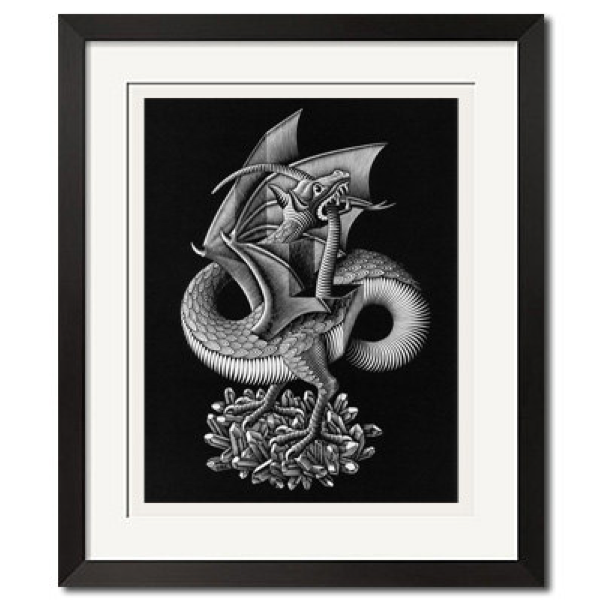
\includegraphics[scale=0.8]{img/Escher-Dragon.eps}
 %\captionsetup{labelformat=empty}
 \caption{埃舍尔《龙》}
 \label{fig:Escher-Dragon}
%\end{figure}
\end{wrapfigure}

我们的理性思维是伟大的。它可以跨越千年,与古代的先哲对话;它可以跨越宇宙,思考我们足迹无法踏上的天体;它可以预见出肉眼看不见的基本粒子;它可以突破直觉,到达高维度的神奇世界。仰望天空,无论是天高云淡,还是月朗星稀,我们也会感叹自身的渺小,在浩瀚的时间长河中,我们不过是匆匆的过客,犹如沧海一粟。

本章我们探讨的问题,究其实质是人类自身的问题。我们的理性思维是否存在边界?我们是否在沿着一个怪圈吞噬着自己?在人工智能突飞猛进发展时,这是每个人都会思考的问题。人类在试图用机器同构自己,用巨大的计算资源同构我们的大脑和理性思维。这就如同埃舍尔作品中的龙,它奋力想从二维世界中挣脱出来,它自己觉得已经把画纸的中部剪开一个缺口,并把尾巴伸了出来。这条龙一口咬住自己的尾巴,拼命想把自己拉到三维的世界中去。作为旁观者的我们,却明明白白知道所有的这一切,仍然在二维的纸张上。这条龙的努力是徒劳的。所有这一切,皆是虚妄、如雾亦如电、当作如是观。

一百年前的激烈讨论和哥德尔的天才证明,在今天依然有着现实意义。作为人类,我们心怀敬畏,敬畏自然,敬畏宇宙,敬畏我们祖先,也敬畏我们自身。

\ifx\wholebook\relax \else
\begin{thebibliography}{99}

\bibitem{Gatys-2015}
Leon A. Gatys, Alexander S. Ecker, Matthias Bethge. ``A Neural Algorithm of Artistic Style.'' 2015. arXiv:1508.06576 [cs.CV] IEEE Conference on Computer Vision and Pattern Recognition (CVPR) 2017.

\bibitem{GuSen-2012}
顾森 《思考的乐趣——Matrix67数学笔记》 人民邮电出版社,2012年,ISBN: 9787115275868

\bibitem{SICP}
Harold Abelson, Gerald Jay Sussman, Julie Sussman 著 裘宗燕 译 ``计算机程序的构造和解释(原书第二版)''. 北京 机械工业出版社 2004年 ISBN: 7-111-13510-5

\bibitem{HanXueTao16}
韩雪涛 ``数学悖论与三次数学危机''. 人民邮电出版社. 2016, ISBN: 9787115430434

\bibitem{M-Kline-2007}
[美] M$\cdot$克莱因 著 李宏魁 译 ``数学:确定性的丧失'' 湖南科学技术出版社,2007年4月 ISBN: 978-7-5357-1857-0
% Morris Kline ``Mathematics: The Loss of Certainty''. Oxford University Press, 1980.

\bibitem{Poincare2}
[法]彭加勒 著,李醒民 译 ``科学的价值'' 商务印书馆. 2010 ISBN: 978-7-100-07045-4

\bibitem{Ried-1996}
[美]康斯坦丝·瑞德 著,袁向东 / 李文林 译 ``希尔伯特:数学界的亚历山大'' 上海科学技术出版社. 2018-8, ISBN: 978-7-5478-4088-7

\end{thebibliography}

\expandafter\enddocument
%\end{document}

\fi
